\chapter[Molten Salt Reactors]{Molten Salt Reactors}


\section{History}
\gls{MSR} development started in the late 1940's as part of the United States' program to design a nuclear powered airplane \cite{bettis_aircraft_1957}. Particularly, liquid fuel appeared to offer a number of advantages, so experiments to demonstrate the feasibility of molten salt fuels were begun in 1947. ``At the enthusiastic urging of Bettis and on the recommendation of W.R. Grimes, R.C. Briant adopted molten fluoride salts in 1950 as the main line effort of the \glsfirst{ORNL}'s Aircraft Nuclear Propulsion program." The fluorides appeared exceptionally suitable because they have high solubility for uranium, are among the most stable of chemical compounds, have low vapor pressure even at temperature more than 1300$^{\circ}$C, have fairly good hydraulic and thermal properties, do not react furiously with air or water, are not damaged by high neutron fluxes, and are inert to some common structural materials \cite{rosenthal_molten-salt_1970}.

A small test reactor, the \gls{ARE}, was built at Oak Ridge site to probe the use of molten fluoride fuels for aircraft propulsion reactors and to study the nuclear stability of the circulating fuel system. The fuel salt for the \gls{ARE} was a mixture of NaF, ZrF$_4$, and UF$_4$. BeO served as moderator, and all the piping was nickel-chromium alloy Inconel. The experiment was successful: in 1954 the \gls{ARE} was operated for 9 days at steady-state outlet temperatures up to 860$^{\circ}$C and at powers up to 2.5 MW$_{(th)}$. No mechanical or chemical problems were observed, and the reactor was found to be stable and self-regulating \cite{bettis_aircraft_1957}.

The great potential of \glspl{MSR} for civilian power application was recognized from the beginning of Aircraft Nuclear Propulsion program, and in 1956 H.G. MacPherson founded a group to study the technical characteristics, nuclear performance, and economics of molten salt converting and breeding reactors. After few years of research with number of concepts, MacPherson and his colleagues concluded that graphite-moderated thermal reactors operating on a thorium fuel cycle would be the best choice for applying molten salt systems for producing economic energy \cite{rosenthal_molten-salt_1970}. Breeding $^{233}$U from $^{232}$Th was found to give better performance in a molten salt thermal reactor neutron energy spectrum than a uranium fuel cycle in which depleted uranium ($^{238}$U) is the fertile material and fissile $^{239}$Pu is produced and recycled. Homogeneous reactor designs that have an entire core consisting liquid salt were rejected because the moderation by the salt was limited compared to a reactor moderated by graphite. Furthermore, intermediate spectrum reactors did not appear to have high enough breeding ratios to compensate their higher inventory of fuel \cite{rosenthal_molten-salt_1970}. Later studies of fast spectrum molten salt reactors have shown that effective breeding could be obtained with extremely high power densities that needed to avoid excessive fissile inventories \cite{kasten_mosel_1964}. Acceptable  power densities appeared challenging to achieve without using novel and untested heat transfer technologies \cite{rosenthal_molten-salt_1970}.

Two types of graphite-moderated reactors were selected by MacPherson's group for further research: single-fluid reactors in which thorium and uranium are dissolved in the same carrier salt, and two-fluid design in which a fertile salt accommodated $^{232}$Th is separated from the fissile salt which contains $^{233}$U and/or $^{239}$Pu as initial fissile load for reactor startup. The two-fluid reactor could operate as breeder except that construction materials for flows separation would significantly deteriorate neutron economy and, consequently, breeding ratio. The single-fluid design is much simplier, easier to build and offers lower power costs, even for that time technology which could only achieve breeding ratio slightly below 1.0. The chemical reprocessing method, namely the fluoride volatility process \cite{cathers_uranium_1957}, which separates uranium from fluoride salts, had been already demonstrated during \gls{ARE} for recovery uranium from \gls{ARE} fuel salt and might be used for partial reprocessing of salts from another type of reactor.

The U.S. Atomic Energy Commission Task Force has considered results of the \gls{ORNL} research and made a comparative evaluation of liquid-fueled reactors early in 1959. One conclusion of the Task Force was that the \gls{MSR} even limited in potential breeding gain, had ``the highest probability of achieving technical feasibility" \cite{noauthor_report_1959}.

In the 1960s more complete conceptual \gls{MSR} designs have been developed. \gls{ORNL} concluded that both single-fluid and two-fluid concepts would lead to reactors with low cost of power generation, and that moving to the breeder either directly or using the converter would create reactors with good fuel utilization characteristics \cite{rosenthal_molten-salt_1970}. Because many of the features of commercial power reactors would differ from those for the \gls{ARE}, and the \gls{ARE} had been operated only a short period of time, new reactor experiment with molten salt was necessary to investigate some of the technology for civilian power reactors.

The developing of the \gls{MSRE} was started in 1960. Creators selected a single-fluid design because it is similar to a converter, but the fuel salt did not contain thorium, and, consequently, was similar to the fuel salt composition for a two-fluid breeder. The \gls{MSRE} fuel salt is a mixture of uranium, $^7$Li, beryllium, and zirconium fluorides. Bare graphite serves as the moderator because the salt cannot penetrate into its pores if the pore sizes are small. Specially developed in the aircraft program, nickel-based alloy INOR-8 (also called Hastelloy-N) for use with molten fluorides was employed as a main constuction material for piping and system components. The maximum power is about 8MW$_{th}$, and the heat is dissipated to the atmosphere \cite{haubenreich_experience_1970}.

Construction of the \gls{MSRE} began in 1962, and the reactor first became critical in 1965. Figure~\ref{fig:msre} shows assembling of a graphite reactor core. Continuous operation at full power began in December 1966. Successful completion of a six-month test campaign in March of 1968 closed the first phase of operation, all initial objectives were achived. The molten fluoride fuel salt was used in the reactor core for many month at temperatures $\geq$649$^{\circ}$C without corrosive damaging of the metal and graphite elements of the system. All reactor equipment worked reliably, radioactive liquids and gases were retained safely, the fuel salt was absolutely stable. Xenon was removed continuously from the salt. Radioactive equipment was repaired or replaced in acceptable time without overexposing maintenance personnel.

The second stage of \gls{MSRE} started in August 1968 when a small chemical processing facility connected to the reactor was used to remove the original uranium from the fuel salt using fluorine gas. $^{233}$U fuel was added to the same carrier salt, and on October 2 the \gls{MSRE} began operation using $^{233}$U. Six days later the power 100 kW was achieved by Glenn T.Seaborg, Chairman of the U.S. Atomic Energy Commission, bringing to power the first reactor in the world to operate using $^{233}$U \cite{haubenreich_experience_1970}.

\begin{figure}[htp!] % replace 't' with 'b' to 
  \centering
  \vspace{-0.3em}
  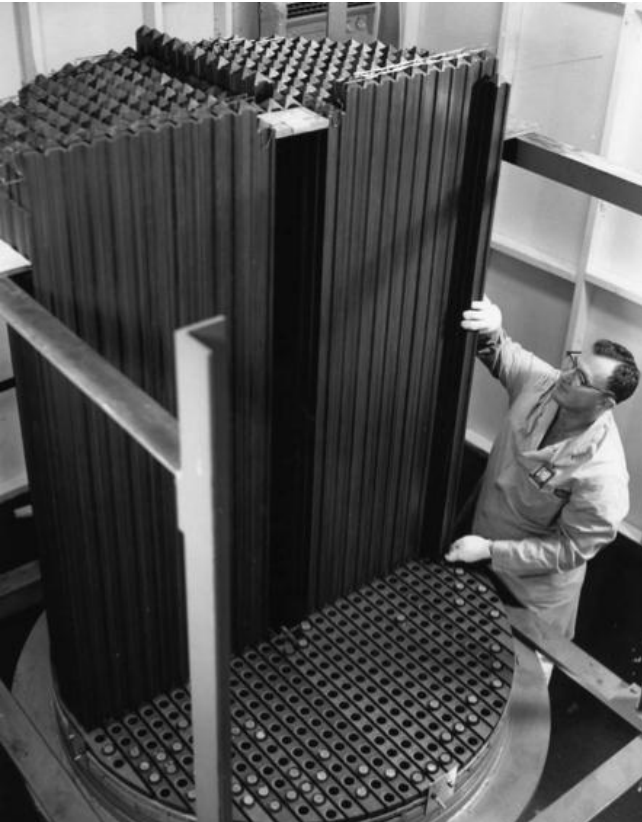
\includegraphics[width=0.75\textwidth]{msre_view.png}
  \caption{The \gls{MSRE} core, shown while being assembled, contains about 1.95 m$^3$ of reactor graphite. The 1'140 fuel channels contain about 0.57m$^3$ of fuel salt.}
  \vspace{-0.6em}
  \label{fig:msre}
\end{figure}
\FloatBarrier

After \gls{MSRE} was built and brought into operation, most of the research and development work on \glspl{MSR} was in support of the \gls{MSRE}. However, molten fluoride salts chemistry continued developing during this period. One discovery during this time was that the lithium fluoride and beryllium fluoride can be separated from rare earths by vacuum distillation at temperature about 1000$^{\circ}$C \cite{kelly_removal_1965}. This method provided an inexpensive, on-site way for recovering valuable rare materials, and following this, the efforts for future reactors changed focus to a two-fluid breeder. In this reactor, the fuel salt should be fluorinated to recover the uranium and distilled to separate carrier salt from fission products. The blanket salt must be processed by fluorination alone, since few fission products would be generated in the blanket if the uranium concentration were kept low \cite{rosenthal_molten-salt_1970}. Graphite tubes in the core were designed to prevent the fuel and fertile streams from mixing.

Two-fluid system analyses have shown that breeding ratio could be in the range of 1.07 to 1.08, which with low fissile inventory would lead to relatively good fuel utilization. Consequently, the development effort for future molten salt reactors by \gls{ORNL} was aimed mainly at the features of two-fluid breeders \cite{briggs_summary_1967}. The main drawback of those reactors was identified as graphite pipes damaging by very high neutron fluxes. Figure~\ref{fig:two_fluid} demostrates design of two-fluid \gls{MSBR} single cell.

Later, in 1967, new experimental information obtained from \gls{MSRE} and an advance in core design lead to shift the \gls{ORNL} molten salt program R\&D focus from the two-fluid to a single-fluid breeder. This switch was based on concerns about graphite behavior at higher radiation exposures that had been achieved previously, graphite changes dimensions more rapidly than had been anticipated. To use in \gls{MSBR} reactor graphite type which was tested during \gls{MSRE}, lower core power densities enabled acceptable graphite lifetime but, even still, these components required frequent replacement. Furthermore, due to core assembly complexity, the entire core and reactor vessel required replacement when any graphite element reached its irradiation limit or developed a leak \cite{rosenthal_molten-salt_1970}.

To achieve acceptable breeding ratio in single-fluid reactor, $^{233}$Pa (27.4-day half-life) must be separated from the fuel salt and held outside the core until it decays to $^{233}$U. Laboratory experiments demonstrated liquid-liquid extraction process for removing protactinium and uranium from molten fluoride salts. The method is to exchange thorium and lithium dissolved in molten bismuth for the components to be removed from the salt. Additional data have confirmed that the uranium can be selectively separated from the salt, the protactinium can be trapped in the salt in a decay tank, and the uranium can be returned back to the fuel salt by electrolysis for subsequent transfer to the core. Analysis indicated that the extraction and electrolysis could be carried out rapidly and continuously.

\begin{figure}[htp!] % replace 't' with 'b' to 
  \centering
  \vspace{-0.3em}
  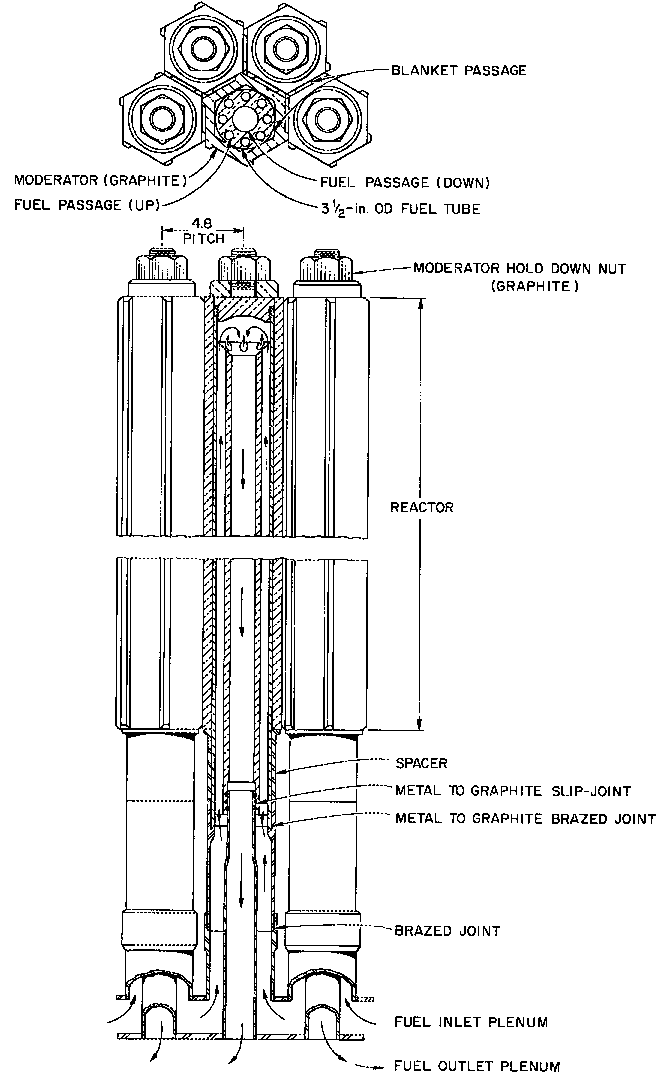
\includegraphics[width=\textwidth]{two_fluid.png}
  \caption{A single graphite ``fuel cell" for a two-fluid molten-salt breeder reactor. Fuel salt flowed upward from the entrance plenum through eight channels at 45-degree angles to one another, then downward through the central channel to the exit plenum \cite{briggs_molten-salt_1966}.}
  \vspace{-0.6em}
  \label{fig:two_fluid}
\end{figure}
\FloatBarrier

The fertile ``blanket'' in the single-fluid breeder is obtained by increasing the volume fraction of fuel salt and reducing the volume fraction of graphite in the outer part of the reactor. This advanced core design makes the outer region undermoderated and increases neutron capture there by the thorium. Moreover, most of neutrons are born in the inner region, at some distance from the reactor boundary, and captures in the outer region which reduce the neutron leakage. Further studies indicated that the fuel utilization in single-fluid, two-region \gls{MSR} can be as good as in two-fluid prototype, and even with the limitation on graphite lifetime the economics might be better \cite{rosenthal_molten-salt_1970}. Thus, in 1968 \gls{ORNL} \gls{MSR} Program was oriented toward the development of single-fluid breeder reactor.

Despite the success of \gls{ARE} and \gls{MSRE}, the \gls{MSR} program closed down in the early 1970s in favor of the liquid metal fast-breeder reactor (LMFBR),\cite{macpherson_molten_1985} after which molten salt reactor research stagnated in the United States. As of 2018, the \gls{ARE} and \gls{MSRE} remained the only \glspl{MSR} ever operated in the world.

Recently, interest in \glspl{MSR} has resurged, with multiple new companies pursuing commercialization of \gls{MSR} designs (e.g. liquid-fueled molten salt designs from Transatomic, Terrapower, Terrestrial, and Thorcon). China initiated a thorium molten salt reactor research project, and demonstrations of the liquid fuel version (TMSR-LF) are targeted for 2024. European Union funds the Safety Assessment of the Molten Salt Fast Reactor (SAMOFAR) project, in which several European research institutes and universities are developing various molten salt reactor prototypes such as the \gls{MSFR}, the \gls{MOSART}, the \gls{FHR}.
To further development of these \gls{MSR} concepts, particularly with respect to their strategies for online reprocessing and refueling, computational analysis methods capturing their unique reactor physics and process chemistry are needed.

\section{Thorium fuel cycle overview}
In the early days of nuclear energy industry, in the United States as a follow-up of the Manhattan Project (1945-1960), leading U.S. national laboratories studied thorium as a possible substitute for uranium and the possibilty of using $^{233}$U in a nuclear weapon. In the Atoms for Peace Program, with its great variety of developments (1955-1975), thorium appeared to be an interesting resource for supplementing limited uranium availability in the context of a fast-growing nuclear industry because thorium is  at least 4-5 times more abundant than uranium in Earth`s crust and preparation of thorium fuel does not require difficult and expensive enrichment processes. International Fuel Cycle Evaluation Conference (INFCE) of 1978 predicted thorium would someday be almost equal in importance to uranium. It stated that in case of the optimistic nuclear energy development scenario, thorium would be called upon massively in the future. These predictions were too optimistic but in a long-term, the use of thorium along with uranium could significantly improve the potential of nuclear energy \cite{lung_perspectives_1998}.

During this pioneering period, thorium fuel cycle research and development for prototype demonstration reactors were initiated, first in the United States under cooperation between the United States Atomic Energy Commission (USAEC) and U.S. industry, then in Europe. About 1500 kg of $^{233}$U have been bred in the United States from 900 metric tons of thorium. Many reactor prototypes as well as thorium extraction plants were built and operated in many countries. The U.S. and France have each separated from the ore about 2000 metric tons of thorium, part of which is still available \cite{lung_perspectives_1998}. However, for most countries uranium was relatively abundant and research in thorium fuel cycles diminished from late 1970s to 2000s. A notable exception was India's three-stage nuclear power program \cite{natarajan_fast_2007}. In the twenty-first century thorium's potential for improving proliferation resistance and waste characteristics is generating renewed interest in the thorium fuel cycle \cite{bagla_thorium_2015}.

Compared to natural uranium which contains 99.284\% $^{238}$U, thorium almost exclusively composed of $^{232}$Th. It can be seen from figure~\ref{fig:th_cycle} that the fertile isotopes are $^{238}$U and $^{232}$Th for uranium-plutonium and thorium fuel cycle, respectively. Accordingly, the fissile isotopes are $^{235}$U, 0.711\% of natural uranium present in nature, and the artificial fissile isotopes are $^{239}$Pu and $^{233}$U for U-Pu and thorium cycles, respectively. 

In the Uranium-Plutonium cycle, production of fissile material ($^{239}$Pu) in a fast-spectrum reactor occurs by neutron irradiation of fertile material ($^{238}$U), while in the thorium fuel cycle $^{232}$Th absorbs a neutron in either a fast or thermal reactor. Next, the $^{233}$Th emits an electron and an anti-neutrino by $\beta^-$ decay to become $^{233}$Pa. The protactinium then emits another electron and anti-neutrino by a second $\beta^-$ decay to become $^{233}$U, which in turn is used as fuel. In \gls{MSR} designs, the $^{233}$Pa is extracted and protected from neutrons (to prevent the core's poisoning via the $^{233}$Pa transmutation into $^{234}$Pa and then to $^{234}$U), until it has decayed to $^{233}$U. Figure~\ref{fig:th_cycle} demonstrates transmutations in the thorium and U-Pu fuel cycles.This is done in order to improve the breeding ratio which is low compared to fast reactors. 

\begin{figure}[t] % replace 't' with 'b' to 
  \centering
  \vspace{-0.3em}
  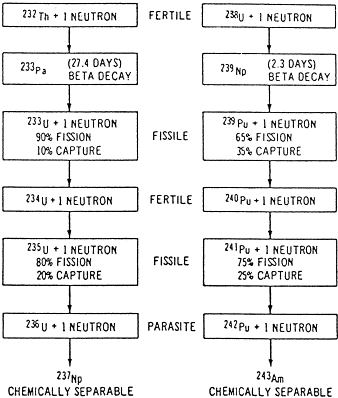
\includegraphics[width=0.70\textwidth]{th_u_cycle.png}
  \caption{Isotopic build-up in $^{232}$Th and $^{238}$U breeding systems \cite{eschbach_possible_1966}.}
  \vspace{-0.6em}
  \label{fig:th_cycle}
\end{figure}
\FloatBarrier

Although the thermal neutron fission cross section ($\sigma_f$) of the resulting $^{233}$U is comparable to $^{235}$U and $^{239}$Pu, it has a much lower capture cross section ($\sigma_c$) than other two fissile isotopes, providing fewer non-fissile neutron absorptions and improving neutron economy. Figure~\ref{fig:n_yeild} shows thermal utilization factor ($\eta$) which in $^{233}$U is greater than other two over a wide range of energies, including the thermal spectrum. Consequently, thorium fuels can be the basis for a thermal breeder reactor \cite{iaea_thorium_2005}, while a breeding reactor in the U-Pu cycle requires a fast neutron spectrum, because, in the thermal spectrum, one neutron absorbed by $^{239}$Pu in average produces less than two neutrons.

Another advantage of the thorium fuel cycle is inherent prolifiration resistance due to contamination of fissile $^{233}$U with $^{232}$U in proposed power reactor designs. $^{232}$U cannot be chemically separated from $^{233}$U and  emits high-energy gamma radiation. These high-energy $\gamma$-rays are a radiological hazard, thus, remote handling is necessary for separated uranium and such materials could be passively detected.

\begin{figure}[htbp!] % replace 't' with 'b' to 
  \centering
  \vspace{-0.3em}
  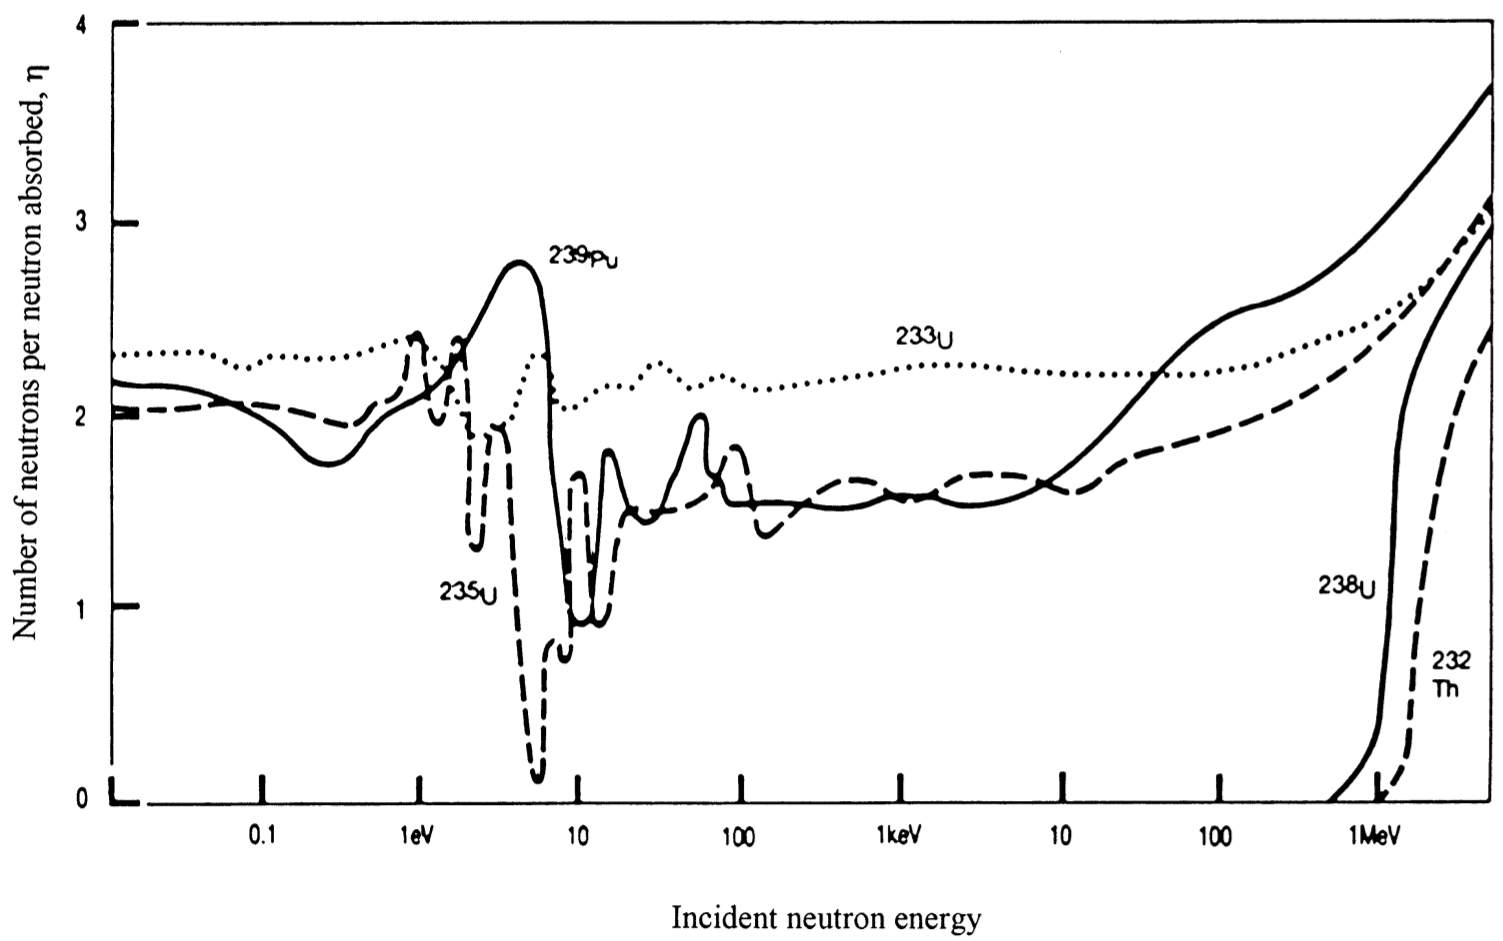
\includegraphics[width=1.05\textwidth]{neutron_yeild.png}
  \caption{Neutron yield per neutron absorbed \cite{anon_plutonium_1989}.}
  \vspace{-0.6em}
  \label{fig:n_yeild}
\end{figure}
\FloatBarrier

Moreover, from the respective positions of uranium and thorium in the periodic table, the long-lived minor actinides resulting from fission are in much lower quantity in the thorium cycle, especially compared with the uranium-plutonium cycle. Because of this, thorium is a potentially attractive alternative to uranium in \gls{MOX} fuels to minimize the generation of long-lived transuranic elements and maximize the destruction of plutonium.

For the many reasons explained above, the thorium fuel cycle has not so far been able to compete on par with uranium, which currently dominates nuclear energy. The time has come to have another hard look at what was perhaps too quickly set aside forty years ago and restart with new advanced computational methods. 

\section{Literature review}
While there is most contemporary nuclear reactor physics software is unable to perform depletion calculations in an online reprocessing regime. Furthermore, no established tool for liquid-fueled \gls{MSR} neutronics and fuel cycle evaluation exist, there are internally developed tools from universities, research institutions for online refueling approximation \cite{serp_molten_2014}. The foundation for these tools was based on early \gls{MSR} simulation methods at \gls{ORNL}, which integrated neutronic and fuel cycle codes \cite{bauman_rod:_1971} into operational plant tools \cite{kee_mrpp:_1976} for \gls{MSR} and reprocessing system design. More recent research efforts in Europe and Asia mainly focus on fast spectrum reactors fuel cycle analysis and use some external tools to couple neutron transport and depletion codes to take into account continuous feeds and removals in \glspl{MSR}. Four of these efforts are listed in table~\ref{tab:fs_codes}.

\begin{table}[h!]
\centering
\caption{Tools and methods for fast spectrum system fuel cycle analysis.}
\begin{tabular}{ |m{0.02\textwidth}|m{0.3\textwidth}|m{0.2\textwidth}|m{0.35\textwidth}|} 
\hline
\# & Neutronic code  & Depletion code    & Authors         \\[5pt]
\hline
1 & \gls{MCNP} \cite{noauthor_mcnp_2004}      & REM \cite{heuer_simulation_2010}  & Doligez \emph{et al.}, 2014; Heuer \emph{et al.}, 2014 \cite{doligez_coupled_2014,heuer_towards_2014}    \\[5pt]
\hline
2 & ERANOS \cite{ruggieri_eranos_2006}      & ERANOS     & Fiorina \emph{et al.}, 2013 \cite{fiorina_investigation_2013}\\[5pt]
\hline
3 & KENO-IV \cite{goluoglu_monte_2011}     & ORIGEN \cite{gauld_isotopic_2011}     & Sheu \emph{et al.}, 2013 \cite{sheu_depletion_2013} \\[5pt]
\hline
4 & SERPENT 2 \cite{leppanen_serpent_2015}   & SERPENT 2  & Aufiero \emph{et al.}, 2013 \cite{aufiero_extended_2013} \\[5pt]
\hline
\end{tabular}
  \label{tab:fs_codes}
\end{table}

Most of these methods are applicable to thermal spectrum reactors, and, additional tools developed specifically for thermal \gls{MSR} applications are listed in table~\ref{tab:th_codes}.

\begin{table}[h!]
\centering
\caption{Tools and approaches for thermal spectrum system fuel cycle analysis.}
\begin{tabular}{ |m{0.02\textwidth}|m{0.2\textwidth}|m{0.2\textwidth}|m{0.45\textwidth}|} 
\hline
\# & Neutronic code  & Depletion code    & Authors         \\[5pt]
\hline
5 & MCODE \cite{xu_mcode_2008}      & ORIGEN2 \cite{croff_users_1980}      & Ahmad \emph{et al.}, 2015 \cite{ahmad_neutronics_2015}     \\[5pt]
\hline
6 & \gls{MCNP}6     & CINDER90 \cite{goorley_mcnp6_2013}     & Park \emph{et al.}, 2015; Jeong \emph{et al.}, 2016 \cite{park_whole_2015, jeong_equilibrium_2016}\\[5pt]
\hline
7 & SCALE \cite{bowman_scale_2011}      & SCALE/ ChemTriton \cite{powers_new_2013}    & Powers \emph{et al.}, 2014; Betzler \emph{et al.}, 2017 \cite{powers_new_2013,powers_inventory_2014,betzler_molten_2017}\\[5pt]
\hline
8 & SERPENT 2      & SERPENT 2     & Rykhlevskii \emph{et al.}, 2017 \cite{rykhlevskii_online_2017} \\[5pt]
\hline
9 & \gls{MCNP}      & REM  & Nuttin \emph{et al.} \cite{nuttin_potential_2005}    \\[5pt]
\hline
\end{tabular}
  \label{tab:th_codes}
\end{table}

Methods (1,3,4) provide some form of reactivity control, and methods (1,4,5,6,8,9) use a set of all nuclides in depletion calculations. 

Liquid-fueled \gls{MSR} designs have online separations and/or feeds, where material is moved to or from the core at all times (continuous) or at specific time steps (batch). To account for batch discharge, a depletion tool should have the capability to remove some or all material at specified interval. This requires the burn-up simulation to stop at a given time and restart with a new liquid fuel composition (after removal of discarded materials and addition of fissile/fertile materials). Accounting for a continuous removal or addition is more difficult because it requires adding a term to the Bateman equations. In SCALE \cite{bowman_scale_2011}, ORIGEN \cite{gauld_isotopic_2011} solves a set of Bateman equations using spectrum-averaged fluxes and cross sections generated from a deterministic transport calculation. Methods (1,4,8) provide opportunity to work with true continuous feeds and removals, while other methods employed batch-wise approach. \gls{ORNL} researchers have developed ChemTriton, Python-based script for SCALE/TRITON which uses a semi-continuous batch process to simulate a continuous reprocessing. This tool models salt treatment, separations, discharge, and refill using an unit-cell \gls{MSR} SCALE/TRITON model over small time steps to simulate continuous reprocessing and deplete the fuel salt \cite{powers_new_2013}.

Thorium-fueled \gls{MSBR}-like reactors similar to the one in this thesis are described in (6,7,8,9). Nevertheless, most of these efforts considered only simplified unit-cell geometry because depletion computations for few year cycle are very computationally expesive even for simple models. 

Nuttin \emph{et al.} broke up reactor core geometry into tree \gls{MCNP} cells: one for salt channels, one for two salt plena above and below the core and the last cell for the annulus, consequently, two-region reactor core was approximated by one region with averaged fuel/moderator ratio \cite{nuttin_potential_2005}.  A similar approach was used by Powers \emph{et al.}, Betzler \emph{et al.}, and Jeong \emph{et al.} \cite{powers_new_2013,powers_inventory_2014,betzler_modeling_2016, betzler_molten_2017, jeong_development_2014, jeong_equilibrium_2016} and clearly misrepresent the two-region breeder reactor concept. The unit-cell or one-region models may produce reliable results for homogeneous reactor cores (i.e. \gls{MSFR}, \gls{MOSART}) or for one-region single-fluid reactor designs (i.e. \gls{MSRE}). A two-region \gls{MSBR} must be simulated using a whole-core model to represent different neutron transport in the inner and outer regions of the core, because most fissions happens in the inner region while breeding occurs in outer zone.  

Aufiero \emph{et al.} extended Monte Carlo burn-up code SERPENT 2 and employed it to study the material isotopic evolution of the \gls{MSFR}. The developed extension directly takes into account the effects of online fuel reprocessing on depletion calculations and features a reactivity control algorithm. The extended version of SERPENT 2 was assessed against a dedicated version of the deterministic ERANOS-based EQL3D procedure \cite{ruggieri_eranos_2006} and adopted to analyze the \gls{MSFR} fuel salt isotopic evolution. We employed this extended SERPENT 2 for a simplified unit-cell geometry of thermal spectrum thorium-fueled \gls{MSBR} and obtained results which contradict existing \gls{MSBR} depletion simulations \cite{jeong_equilibrium_2016}.

Chapter 3 and 4 of current study are mostly similar to the works described in (6,7,9), but the focus of this work is on developing new external open-source tool for online reprocessing simulation named Saltproc. The tool works with Monte Carlo code SERPENT 2, and has a reactivity control module which allows reactivity adjustment by changing feed material flow to avoid control rod movement. Moreover, this work extends recent research efforts by using for online reprocessing simulation high-fidelity full-core 3-D model without any approximations in the core geometry.

Another challenge presented by liquid-fueled systems is the fuel material movement. Fuel flow is important because of delayed neutron emission. In a reactor with solid fuel, the delayed neutron precursor fission products remain very close to the location where fission happened, later emitting delayed neutrons at that location. Delayed neutrons have softer energy spectrum than prompt neutrons \cite{betzler_molten_2017}. In case of liquid-fuled reactors the precursors drifting, consequently, the fission and delayed neutron emission locations are different. The reactor design determines the effect of the precursor drift on the core physics. The flow parameters (e.g., flow rate, pipe diameter, primary loop length) affect on the effective delayed neutron fraction $\beta_{eff}$. This quantity has significant impact on reactor safety because delayed neutron production occurs on a relatively long time frame and enables control of the reactor. Hence, to take into account tightly coupled \gls{MSR} neutronics, thermal-hydraulics, and precursors drift a multi-physics code is required.

There are number of multi-physics tools which successfully describe steady-state and transient behavior of various \gls{MSR} concepts. Krepel \emph{et al.} extended the \gls{LWR} diffusion code DYN3D to consider drift of delayed neutron precursors alongside the reactor temperature profile, re-introducing the extended code as DYN3D-MSR \cite{krepel_dyn3d-msr_2007}. That work compared DYN3D-MSR against experimental \gls{MSRE} data to simulate local fuel channel blockage accidents as well as local temperature perturbations.

Similarly, Kophazi \emph{et al.} used iterative coupling between three-dimensional neutronic and one-dimensional heat conduction models DALTON and THERM to analyze normal \gls{MSRE} operation as well as channel-blocking-incident transients \cite{kophazi_development_2009}. The Kophazi model added entrance effects of heat transfer coefficients as well as thermal coupling between fuel channels through moderator heat conduction. Later, Cammi \emph{et al.} performed a 2D-axisymmetric single-channel analysis of the \gls{MSBR} using the commercial finite element package COMSOL Multiphysics \cite{cammi_multi-physics_2011}. That work directly solved the fuel salt velocity field, and used heterogeneous group constants in fuel and moderator regions.  

More recently, Aufiero \emph{et al.} \cite{aufiero_development_2014} approached transient simulations in the \gls{MSFR} with the finite volume OpenFOAM multiphysics toolkit \cite{weller_tensorial_1998}.  This approach benefits from pre-implemented turbulence models available in the OpenFOAM library and captures the full-core three-dimensional geometry of the reactor primary circuit.  OpenFOAM \gls{CFD} has additionally been shown by Laureau \emph{et al.} \cite{laureau_transient_2017} to couple well with Transient Fission Matrix neutronics within the \gls{MSFR}.

Concurrently, Lindsay \emph{et al.} have introduced Moltres, a physics application for multiphysics modeling of liquid-fueled \glspl{MSR} \cite{lindsay_introduction_2018}. It couples equations for neutron diffusion, thermal-hydraulics, and delayed neutron precursor transport. Moltres solves arbitrary-group neutron diffusion, temperature, and precursor governing equations in anywhere from one to three dimensions and can be deployed on an arbitrary number of processing units. That work compared 2D-axisymmetric many-channel anlysis of the \gls{MSRE} in Moltres against experimental \gls{MSRE} data in steady-state mode.

On the whole, these research efforts used initial fuel salt composition, thus, considering the reactor core at the moment of startup. Nevertheless, fuel salt composition evolves significantly during fuel materials irradiation which leads to changes in the reactor neutronics. Chapter 5 of the present thesis introduces the equilibrium fuel salt composition and compare major reactor physics characteristics for both initial and equilibrium state. This results are necessarily for multi-physics analysis of accident transient scenarios for \gls{MSBR} using Moltres code for both fresh and irradiated fuel salt.

